\documentclass[xcolor=pdftex,romanian,colorlinks]{beamer}

\usepackage{../tslides}
\usetikzlibrary{matrix}
\usepackage{wrapfig}

\title[PD---echivalență]{Echivalență între programe}
\subtitle{Când un fragment de program poate fi înlocuit cu altul?}
\begin{document}
\maketitle

\begin{frame}{Echivalență semantică}{Exemplul I}

{\LARGE \[2 + 2 \stackrel{?}{\simeq} 4\] }


\onslide<2>
\begin{itemize}
\item Sunt echivalente cele două expresii? În ce sens?
\item Au arbori de sintaxă diferiți
\item Au secvențe de rescriere diferite
\item Dar e destul de clar putem înlocui $2+2$ cu $4$ oriunde în orice program
\[\int_0^{2+2}{e^{\sin(x)}}dx = \int_0^4{e^{\sin(x)}}dx\]
\end{itemize}

\end{frame}


\begin{frame}{Echivalență de cod}{Exemplul II}

\begin{block}{\large $l \terminal{:=} 0 \terminal{;} 4 \stackrel{?}{\simeq} l \terminal{:=} 1 \terminal{;} 3 \terminal{+} !l$ }

\begin{itemize}
\item<2-> Dacă le evaluăm în orice stare, obținem aceeași valoare.
\item<3-> Dar \alert{nu} putem să înlocuim o expresie cu cealaltă într-un context arbitrar.
\item<4> De exemplu, fie contextul $C[\_] = \_ + !l$. Avem că
$\begin{array}{ccc}
C[l \terminal{:=} 0 \terminal{;} 4] & = &(l \terminal{:=} 0 \terminal{;} 4) + !l \\
&&\displaystyle \not\simeq\\ 
C[l \terminal{:=} 1 \terminal{;} 3 \terminal{+} !l] & = & (l \terminal{:=} 1 \terminal{;} 3 \terminal{+} !l) + !l
\end{array}$
\end{itemize}
\end{block}
\begin{block}{Alte exemple}
\begin{itemize}
\item $l \terminal{:=} !l + 1 \terminal{;} l \terminal{:=} !l + -1 \stackrel{?}{\simeq} l \terminal{:=} !l$
\item $ l \terminal{:=} !l + 1 \terminal{;} l \terminal{:=} !l + -1 \stackrel{?}{\simeq} \Sskip$
\end{itemize}
\end{block}
\end{frame}


\begin{frame}{Echivalența de cod}
\begin{block}{Intuiție}
Două „fragmente“ de cod $e_1$ și $e_2$ sunt \structure{echivalente} dacă „au același efect“ \structure{în orice context} ar fi folosite.
\end{block}

\vfill \begin{block}{Utilitate}
\begin{itemize}
\item Stabilirea echivalenței poate fi f. utilă în procesul de compilare
\item Permite înlocuirea unei bucăți de cod cu alta mai „bună“ 
\end{itemize}
\end{block}

\end{frame}

\begin{frame}{Mai multe exemple (parametrizate)}
\begin{itemize}
\item $e_1 \terminal{;} (e_2 \terminal{;} e_3) \stackrel?\simeq (e_1 \terminal{;} e_2) \terminal{;} e_3$
\vitem $e_1 \terminal{;} e_2 \stackrel?\simeq e_2 \terminal{;} e_1$
\vitem $e \terminal{;} {\Sif b \Sthen e_1 \Selse e_2}  \stackrel?\simeq {\Sif b \Sthen (e \terminal{;} e_1) \Selse (e \terminal{;} e_2)}$
\vitem $({\Sif b \Sthen e_1 \Selse e_2}) \terminal{;} e  \stackrel?\simeq {\Sif B \Sthen (e_1 \terminal{;} e) \Selse (e_2 \terminal{;} e)}$
\end{itemize}

\end{frame}


\begin{frame}{Exemplu mai complexe (parametrizat)}
\[\begin{array}{c}\Slet x = \Sref 0 \Sin {\Sfun (y:\Sint) \rightarrow x \terminal{:=} !x + y \terminal{;} !x}
\\
\stackrel{?}{\simeq}
\\
\Slet x = \Sref 0 \Sin {\Sfun (y:\Sint) \rightarrow x \terminal{:=} !x - y \terminal{;} 0 - !x}
\end{array}\]


\end{frame}

\begin{frame}{De ce semantică}
Definițiile semantice ne ajută să 
\begin{enumerate}
\item Definim clar/formal noțiunea de echivalență
\item Analizăm matematic echivalența între bucățile de cod
\begin{itemize}
\item Identificarea precisă a condițiilor în care echivalența ține
\item Demonstrarea echivalenței
\end{itemize}
\end{enumerate}
\end{frame}


\begin{section}{Echivalență semantică}


\begin{frame}{Proprietăți dezirabile ale echivalenței de cod}{Relație de congruență}
\begin{description}
\item[Reflexivitate] \hfill $\displaystyle \reg{P \simeq P}{}{}$ \hfill\;
\vitem[Simetrie] \hfill $\displaystyle \reg{P \simeq P'}{P' \simeq P}{}$ \hfill\;
\vitem[Tranzitivitate] \hfill $\displaystyle \reg{P \simeq P''}{P \simeq P' \si P' \simeq P''}{}$ \hfill\;
\vitem[Congruență] \hfill \structure{$\displaystyle \reg{{\cal C}[P] \simeq {\cal C}[P']}{P \simeq P'}{}$} \hfill\;
\end{description}
\vfill
pentru orice $P, P', P''$ fraze de program și $\cal C$ \structure{context}.
\vfill
\begin{itemize}
\item[] \structure{${\cal C}[P]$} —frază de program cu o apariție a lui $P$ evidențiată
\item[] \structure{${\cal C}[P']$} —aceeași frază în care apariția lui $P$ a fost înlocuită cu $P'$
\end{itemize}
\end{frame}



\begin{frame}<handout:0|article:0>{Echivalență semantică}

\begin{block}{Intuiție}
Două programe sunt echivalente dacă se evaluează la fel.
\end{block}

\begin{block}{Definiție}
Două expresii $e_1$ și $e_2$ sunt echivalente semantic, notat $e_1 \simeq e_2$ dacă pentru orice stări $s$ și $s'$ și valoare $v$,
\[{\c{e_1,s}}\longrightarrow^\ast{\c{v,s'}} \iff {\c{e_2,s}}\longrightarrow^\ast{\c{v,s'}}\] 
\end{block}
\end{frame}

\begin{frame}{\only<beamer>{Echivalență semantică în IMP}}{Exemple}
\begin{itemize}
\item $e \simeq {\Sskip}\terminal{;} e$ 
\item dacă $\vdash e : \Sunit$, atunci $e\terminal{;} {\Sskip} \simeq e$
\vitem $e_1 \terminal{;} (e_2 \terminal{;} e_3) \simeq (e_1 \terminal{;} e_2) \terminal{;} e_3$ 
\vitem $({\Sif b \Sthen e_1 \Selse e_2}) \terminal{;} e  \simeq {\Sif b \Sthen (e_1 \terminal{;} e) \Selse (e_2 \terminal{;} e)}$ 
\vitem $\Sif {\Strue} \Sthen e_1 \Selse e_2 \simeq e_1$
\vitem $\Sif {\Sfalse} \Sthen e_1 \Selse e_2 \simeq e_2$
\vitem $\Swhile  b \Sdo e \Sdone \simeq {\Sif b \Sthen (e \terminal{;} {\Swhile  b \Sdo e \Sdone}) \Selse {\Sskip}}$
\vitem $l_1 \terminal{:=} n_1 \terminal{;} l_2 \terminal{:=} n_2\simeq \left\{\begin{array}{lll} l_2 \terminal{:=} n_2 \terminal{;} l_1 \terminal{:=} n_1 & \textbf{dacă} & l_1 \neq l_2
\\ l_2 \terminal{:=} n_2 & \textbf{dacă} & l_1 = l_2 \end{array}\right.$ 
\end{itemize}
\end{frame}



\begin{frame}{\only<beamer>{Echivalența semantică pentru limbajul IMP}}
\begin{block}{Observație}
Definiția dată pentru echivalență nu distinge între execuțiile care se blochează 
\begin{itemize}
\item operație aritmetică imposibilă (împărțire la 0)
\item accesarea unei locații indisponibile
\item ne-terminarea execuției
\end{itemize}
\end{block}

\vfill
\begin{block}{Exercițiu}
Dați exemplu de două expresii a căror execuție poate eșua în mod diferit, dar care sunt totuși echivalente.
\end{block}
\end{frame}


\begin{frame}{Ne-echivalența semantică $\not\simeq$}

\begin{block}{Modalitate de demonstrare — contraexemplul}
	Pentru a arăta (de exemplu că) $e_1\not\simeq e_2$, e suficient să găsesc niște stări de memorie $s$ și $s'$ și o valoare $v$ astfel încât:
\[\Ss{\c{e_1,s}}{\!\!^\ast\,\c{v,s'}} \textbf{ și }\c{e_2,s} \not\rightarrow^\ast \c{v,s'}\]
(sau invers)
\end{block}

\begin{block}{Exemplu}
E adevărat că pentru orice expresii $b, e, e_1, e_2$ și orice expresie booleană $e$,
\[{ e \terminal{;}{\Sif b \Sthen e_1 \Selse e_2}}  \simeq {\Sif b \Sthen (e \terminal{;} e_1) \Selse (e \terminal{;} e_2)}\mbox{ ?}\]
\end{block}
\end{frame}

\end{section}

\begin{section}{Echivalență observațională}

\begin{frame}[fragile]{Care din următoarele programe sunt echivalente?}
{IMP + I/O}
\begin{block}{}
\hfill\begin{minipage}[t]{.3\columnwidth}
\begin{asciiml}
let l = ref 0 in
while true do 
 l := read_int () ;
 print_int(!l 
         - read_int())
done

      (a)
\end{asciiml}
\end{minipage}
\hfill\begin{minipage}[t]{.3\columnwidth}
\begin{asciiml}
while true do 
  print_int(read_int() 
          - read_int())
done


      (b)
\end{asciiml}
\end{minipage}
\hfill\begin{minipage}[t]{.3\columnwidth}
\begin{asciiml}
let l = ref 0 in
while true do 
  l := read_int() ;
  print_int(read_int() 
          - !l)
done

      (c)
\end{asciiml}
\end{minipage}
\end{block}

\onslide<2>
\begin{itemize}
\item Conform echivalenței semantice cele trei programe sunt echivalente
\begin{itemize}
\item Nici unul nu se evaluează la nici o valoare nicicând
\end{itemize}
\item Vrem să putem demonstra că (a) și (b) \structure{se comportă} la fel
\item Vrem să putem demonstra că (c) \structure{se comportă} diferit de (a) și (b)
\end{itemize}
\end{frame}

\begin{subsection}{Simulare}
\begin{frame}{\only<beamer|handout>{Simulare}}
\begin{block}{Intuiție}
Un program $q$ îl simulează pe un altul $p$ dacă oricând $p$ poate face un pas observabil, poate și $q$ să facă același pas (modulo mai mulți pași $\epsilon$).
\end{block}

\begin{block}{Definiție}
O \structure{simulare} pentru sistemul de tranziție cu etichete $({\it Config}, {\it Act}, \rightarrow)$ este o relație ${\cal R} \subseteq {\it Config} \times {\it Config}$ cu proprietatea că pentru orice două configurații $c_1, c_2$, dacă $c_1 \mathrel{\cal R} c_2$ și $\Ss[\alpha]{c_1}{c_1'}$, atunci există $c_2'$ astfel încât $c_1 \mathrel{\cal R} c_2$ și $\Ss[\hat{\alpha}]{c_2}{c_2'}$, unde: 

\[\Ss[\hat{\alpha}]{c}{c'} = \left\{\begin{array}{ll}
\Ss[\epsilon^\ast]{c}{c'} & \mbox{ dacă } \alpha = \epsilon 
\\
\Ss[\epsilon^\ast\alpha\epsilon^\ast]{c}{c'} & \mbox{ altfel }
\end{array}\right.\]

\end{block}
\end{frame}

\begin{frame}{Reprezentare grafică}

\[
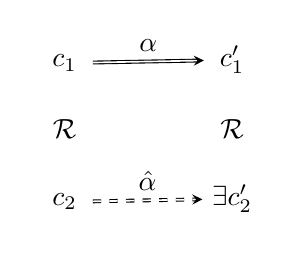
\begin{tikzpicture}[ampersand replacement=\&]
  \matrix(m)[matrix of math nodes,row sep=1em,column sep=4em,minimum width=2em]
  {  c_1 \& c_1' \\
    {\cal R} \& {\cal R} \\
    c_2 \& \exists c_2' \\};
  \path[-stealth]
    (m-1-1) edge [double] node [above] {$\alpha$}  (m-1-2) 
                  %edge [draw=white] node [left] {f} (m-2-1)
 %   (m-1-2) edge node [right] {g} (m-2-2)
    (m-3-1) edge [double, dashed] node [above] {$\hat{\alpha}$} (m-3-2)
   %               edge [bend left=90] (m-1-2)
    %              edge [dashed, bend right=90] (m-1-2)
    ;
\end{tikzpicture}
\]

\[{\cal R}^{-1} \mathrel{;} {\xrightarrow{\alpha}} \subseteq   {\xrightarrow{\hat{\alpha}}}  \mathrel{;} {\cal R}^{-1}\]

\vfill

\begin{block}{Definiție echivalentă}
 $\cal R$ simulare dacă și numai dacă ${\cal R}^{-1} \mathrel{;} {\xrightarrow{\alpha}} \subseteq   {\xrightarrow{\hat{\alpha}}}  \mathrel{;} {\cal R}^{-1}$.  Adică, 
\[c_2 \mathrel{{\cal R}^{-1}} c_1 \xrightarrow{\alpha} c_1'  \implies (\exists c_2')
c_2 \xrightarrow{\hat{\alpha}} c_2' \mathrel{{\cal R}^{-1}} c_1' \]
\end{block}
\end{frame}



\begin{frame}{Simularea între programe}{Definiții}
\begin{itemize}
\item O configurație $c_1$ \structure{este simulată} de o configurație $c_2$, notat \structure{$c_1 \leq c_2$} dacă există o simulare $\cal R$ astfel încât $c_1 \mathrel{\cal R} c_2$.

\vitem O expresie $e_1$ \structure{este simulată} de o expresie $e_2$, notat $e_1 \leq e_2$ dacă pentru orice stare a memoriei $s$,  $\c{e_1,s}\leq \c{e_2,s}$
\end{itemize}

\begin{block}{Intuiție}
$e_2$ îl simulează  pe $e_1$ dacă, în orice moment al execuției, oricând $e_1$ poate să efectueze o acțiune, poate și $e_2$ să facă același lucru.
\end{block}
\end{frame}

\begin{frame}[fragile]{Exemplu}{Arătați că}
\ 

\hfill\begin{minipage}{.42\columnwidth}
\begin{asciiml}
let x = ref 3 in
while 0 <= !x do 
  x := !x - 1 ;
  print_int(read_int() - read_int())
done
\end{asciiml}
\end{minipage}
\hfill\begin{minipage}{.05\columnwidth}
\LARGE \[\leq\]
\end{minipage}
\hfill\begin{minipage}{.42\columnwidth}
\begin{asciiml}
while true do 
  print_int(read_int() - read_int())
done
\end{asciiml}
\end{minipage}
\end{frame}

\begin{frame}{Proprietăți}{Definiții echivalente}
\begin{enumerate}
\item
${\cal R}$ simulare dacă și numai dacă oricând $c_1\mathrel{\cal R} c_2$ și $\Ss[\hat{\alpha}]{c_1}{c_1'}$, există $c_2'$ astfel încât $c_1' \mathrel{\cal R} c_2'$ și $\Ss[\hat{\alpha}]{c_2}{c_2'}$.

\vitem $\cal R$ simulare dacă și numai dacă ${\cal R}^{-1} \mathrel{;} {\xrightarrow{\hat{\alpha}}} \subseteq   {\xrightarrow{\hat{\alpha}}}  \mathrel{;} {\cal R}^{-1}$.  Adică, 
\[c_2 \mathrel{{\cal R}^{-1}} c_1 \xrightarrow{\hat{\alpha}} c_1'  \implies (\exists c_2')
c_2 \xrightarrow{\hat{\alpha}} c_2' \mathrel{{\cal R}^{-1}} c_1' \]

\vitem $\cal R$ simulare dacă și numai dacă oricând $c_1\mathrel{\cal R} c_2$ și $\Ss[\hat{w}]{c_1}{c_1'}$, există $c_2'$ astfel încât $c_1' \mathrel{\cal R} c_2'$ și $\Ss[\hat{w}]{c_2}{c_2'}$, unde $\xrightarrow{\hat{w}}$ este extensia canonică a lui $\xrightarrow{\hat{\alpha}}$ la cuvinte peste alfabetul actiunilor.
\end{enumerate}
\end{frame}

\begin{frame}{Reprezentare grafică a simulării}
\large
\[
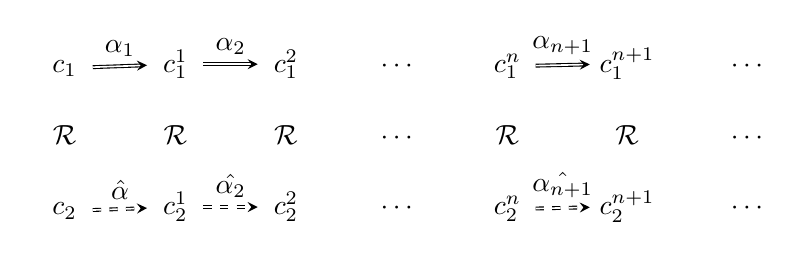
\begin{tikzpicture}[ampersand replacement=\&]
  \matrix(m)[matrix of math nodes,row sep=1em,column sep=2em,minimum width=2em]
  {  c_1 \& c_1^1 \& c_1^2 \& \cdots \& c_1^n \& c_1^{n+1} \& \cdots \\
    {\cal R} \& {\cal R}  \& {\cal R} \& \cdots \& {\cal R} \& {\cal R} \&\cdots\\
c_2 \& c_2^1 \& c_2^2 \& \cdots \& c_2^n \& c_2^{n+1} \& \cdots \\
};
  \path[-stealth]
    (m-1-1) edge [double] node [above] {$\alpha_1$}  (m-1-2) 
    (m-1-2) edge [double] node [above] {$\alpha_2$}  (m-1-3) 
    (m-1-5) edge [double] node [above] {$\alpha_{n+1}$}  (m-1-6) 
    (m-3-1) edge [double, dashed] node [above] {$\hat{\alpha}$} (m-3-2)
    (m-3-2) edge [double, dashed] node [above] {$\hat{\alpha_2}$} (m-3-3)
    (m-3-5) edge [double, dashed] node [above] {$\hat{\alpha_{n+1}}$} (m-3-6);
\end{tikzpicture}
\]
\end{frame}

\end{subsection}
\begin{subsection}{Bisimulare}
\begin{frame}{\only<handout|beamer>{Bisimulare}}
\begin{block}{Definiție}
O \structure{bisimulare} pentru sistemul de tranziție cu etichete $({\it Config}, {\it Act}, \rightarrow)$ este o relație ${\cal R} \subseteq {\it Config} \times {\it Config}$ cu proprietatea că pentru orice două configurații în relația \structure{$c_1 \mathrel{\cal R} c_2$} avem:
\begin{itemize}
\item  
Dacă $\Ss[\alpha]{c_1}{c_1'}$, atunci există $c_2'$ astfel încât $c_1' \mathrel{\cal R} c_2'$ și $\Ss[\hat{\alpha}]{c_2}{c_2'}$. 
\item  
Dacă $\Ss[\alpha]{c_2}{c_2'}$, atunci există $c_1'$ astfel încât  $c_1' \mathrel{\cal R} c_2'$ și $\Ss[\hat{\alpha}]{c_1}{c_1'}$. 
\end{itemize}

Adică ${\cal R}$ bisimulare dacă și numai dacă atât ${\cal R}$, cât și ${\cal R}^{-1}$ sunt simulări. 
\end{block}
\end{frame}



\begin{frame}{Bisimulare}{Reprezentare grafică}

\hfill\begin{minipage}{.3\columnwidth}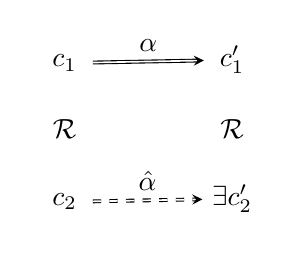
\begin{tikzpicture}[ampersand replacement=\&]
  \matrix(m)[matrix of math nodes,row sep=1em,column sep=4em,minimum width=2em]
  {  c_1 \& c_1' \\
    {\cal R} \& {\cal R} \\
    c_2 \& \exists c_2' \\};
  \path[-stealth]
    (m-1-1) edge [double] node [above] {$\alpha$}  (m-1-2) 
                  %edge [draw=white] node [left] {f} (m-2-1)
 %   (m-1-2) edge node [right] {g} (m-2-2)
    (m-3-1) edge [double, dashed] node [above] {$\hat{\alpha}$} (m-3-2);
\end{tikzpicture}

\[{\cal R}^{-1} \mathrel{;} {\xrightarrow{{\alpha}}} \subseteq   {\xrightarrow{\hat{\alpha}}}  \mathrel{;} {\cal R}^{-1}\]
\end{minipage}
\hfill\mbox{\LARGE și }
\hfill \begin{minipage}{.3\columnwidth}
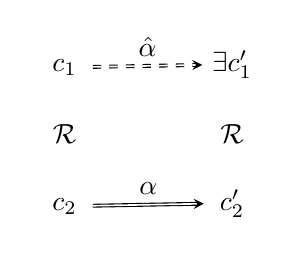
\begin{tikzpicture}[ampersand replacement=\&]
  \matrix(m)[matrix of math nodes,row sep=1em,column sep=4em,minimum width=2em]
  {  c_1 \&\exists  c_1' \\
    {\cal R} \& {\cal R} \\
    c_2 \& c_2' \\};
  \path[-stealth]
    (m-1-1) edge [double, dashed] node [above] {$\hat{\alpha}$}  (m-1-2) 
                  %edge [draw=white] node [left] {f} (m-2-1)
 %   (m-1-2) edge node [right] {g} (m-2-2)
    (m-3-1) edge [double] node [above] {$\alpha$} (m-3-2);
\end{tikzpicture}

\[{\cal R} \mathrel{;} {\xrightarrow{{\alpha}}} \subseteq   {\xrightarrow{\hat{\alpha}}}  \mathrel{;} {\cal R}\]
\end{minipage}
\hfill\ 

\end{frame}

\begin{frame}{Bisimularea între programe}{Definiții}
\begin{itemize}
\item O configurație $c_1$ \structure{este bisimulată} de o configurație $c_2$, notat \structure{$c_1 \approx  c_2$} dacă există o bisimulare $\cal R$ astfel încât $c_1 \mathrel{\cal R} c_2$.

\vitem O expresie $e_1$ \structure{este bisimulată} de o expresie $e_2$, notat $e_1 \approx e_2$ dacă pentru orice stare a memoriei $s$,  $\c{e_1,s}\approx \c{e_2,s}$
\end{itemize}

\vfill
\begin{alertblock}{Observație}
$e_1 \approx e_2$ implică $e_1 \leq e_2$ și $e_2 \leq e_1$, dar reciproca nu este tot timpul validă.
\end{alertblock}
\end{frame}




\begin{frame}[fragile]{Vrem putem să demonstrăm}
\hfill\begin{minipage}{.25\columnwidth}
\begin{asciiml}


while true do 
  l := read_int() ;
  print_int(!l
          - read_int())
done
\end{asciiml}
\end{minipage}
\hfill{\Large $\approx$}\hfill\begin{minipage}{.25\columnwidth}
\begin{asciiml}


while true do
  print_int(read_int()
          - read_int())
done

\end{asciiml}
\end{minipage}
\hfill{\Large $\not\approx$}\hfill\begin{minipage}{.25\columnwidth}
\begin{asciiml}


while true do
  l := read_int() ;
  print_int(read_int()
          - !l)
done
\end{asciiml}
\end{minipage}
\hfill\ 

\end{frame}

\end{subsection}

\end{section}

\end{document}